%%%%%%%%%%%%%%%%%%%%%%%%%%%%%%%%%% Chapter 5 %%%%%%%%%%%%%%%%%%%%%%%%%%%%%%%%%%
\chapter{Implementation \label{chapter:5}}
    With almost every expression given in \Arf{chapter:3} being some kind of
    sum it is not hard to imagine that solving them by hand would be quite the
    challenge and most likely\footnote{Read definitely.} impossible, but with
    the modern computer at our disposal they can be tackled numerically.
    However in order to get the data from the numerical simulations the actual
    implementation, the raw code, has to be written, tested, verified and run. \\
    This chapter will explain the code used in the thesis in detail. The main
    code base is given in \url{https://github.com/Oo1Insane1oO/HartreeFock} and
    \url{https://github.com/Oo1Insane1oO/VMC}. General information of the usage
    of packages are given in appendix >> REF APPENDIX << while the structure
    and workflow of the code is given here. We will first present a
    workflow-chart of the two main code-bases used, namely the Hartree-Fock
    implementation and the Variational Monte-Carlo implementation.
    \begin{figure}[H]
        \centering
        \begin{tikzpicture}[
                >={Latex[width=2mm,length=2mm]},
                    base/.style = {rectangle, rounded corners, draw=black,
                                minimum width=2cm, minimum height=0.5cm, text
                                centered, font=\sffamily},
                    basecode/.style = {rectangle, rounded corners, draw=black,
                                minimum width=2cm, minimum height=0.5cm, text
                                centered, font=\sffamily, align=left},
                    activityStarts/.style = {base, fill=NavyBlue!30, drop shadow},
                    startstop/.style = {base, fill=Maroon!25, drop shadow},
                    startstopcode/.style = {basecode, fill=Maroon!25, drop shadow},
                    activityRuns/.style = {base, fill=ForestGreen!25, drop shadow},
                    process/.style = {base, fill=white!15, font=\sffamily, drop shadow},
                    processcode/.style = {basecode, fill=white!15, font=\sffamily, drop shadow},
                scale=0.8, 
                node distance=1.5cm, 
                every node/.style={fill=white, font=\sffamily},
                align=center]
            \node (main) [activityStarts] {Main};
            \node (make) [activityRuns, right of=main, xshift=3.5cm] {
               run make with flag \\
               make BASIS=SYSTEM
            };
            \node (compilation) [activityRuns, right of=make, xshift=3cm] {
                Compilation
            };
            \node (chooseBasis) [process, above of=compilation] {
                Choose system flag
            };
            \node (HO) [process, left of=chooseBasis, xshift=-3.5cm] {
                HARMONICOSCILLATOR
            };
            \node (DW) [process, above of=chooseBasis] {
               DOUBLEWELL 
            };
            \draw[-] (HO) -- (chooseBasis);
            \draw[-] (DW) -- (chooseBasis);
            \node (arr) [right of=main, xshift=0.3cm] {
                $\Longleftarrow$
            };
            \node (initIntegral) [activityStarts, below of=main] {
                Read YAML file \\ 
                Initialize Integral Object 
                \\ Iterate};
            \node (integralcode) [processcode, right of=initIntegral, xshift=6cm] {
                \lstinline[language=C++, style=ccstyle]{Integral$^*$ HFS = new Integral(D, L, N);} \\
                \lstinline[language=C++, style=ccstyle]{string message = HFS$\rarr$initializeParameters(...);}};
            \node (intcodeexplan) [process, below of=integralcode] {
                \hltexttt{Integral} is one of
            };
            \node (harmonic) [process, below left of=intcodeexplan, xshift=-1cm] {
                \hltexttt{HarmonicOscillator}
            };
            \node (doublewell) [process, below right of=intcodeexplan, xshift=1cm] {
                \hltexttt{DoubleWell}
            };
            \node (iteratecode) [startstop, below of=initIntegral, yshift=-2cm] {
                Calculate integral elements
            };
            \node (assemble) [startstopcode, right of=iteratecode, xshift=6cm] {
                \lstinline[language=C++, style=ccstyle]{assemble();}
            };
            \node (onebody) [startstop, below of=assemble] {
                Calculate $\Braket{p|h|q}$ (only for root)
            };
            \node (obspec) [process, left of=onebody, xshift=-6cm] {
                Using function \hltextttf{oneBodyElement} \\
                in \hltexttt{Integral}
            };
            \node (twobody) [startstop, below of=onebody] {
                Calculate $\Braket{pq|h|rs}$ (in parallel)
            };
            \node (tbspec) [process, left of=twobody, xshift=-6cm] {
                Using function \hltextttf{coulombElement} \\
                in \hltexttt{Integral}
            };
            \node (hfalgo) [process, below of=twobody, yshift=-1cm] {
                Run Hartree-Fock Algorithm
            };
            \node (hfloopstart) [startstop, left of=hfalgo, xshift=-6cm] {
                while $i<\text{maxiteration}$ \\
                    Set Fock-Matrix with \Arf{eq:FockRestrictedDef} \\
                    Solve eigenvalue \Arf{eq:eigvalrestr} \\
                    Set density matrix with \Arf{eq:densitymatrixdef} \\
                    Break if converged
            };
            \node (finish) [activityStarts, below of=hfalgo] {
                Output $E_0$ \\
                free HFS object \\
                Finalize MPI
            };
            \draw[-] (compilation) -- (chooseBasis);
            \draw[<-] (make) -- (compilation);
            \draw[->] (main) -- (initIntegral);
            \draw[<-] (initIntegral) -- (integralcode);
            \draw[-] (integralcode) -- (intcodeexplan);
            \draw[-] (intcodeexplan) -- (harmonic);
            \draw[-] (intcodeexplan) -- (doublewell);
            \draw[->] (initIntegral) -- (iteratecode);
            \draw[<-] (onebody) -- (obspec);
            \draw[<-] (twobody) -- (tbspec);
            \draw[->] (iteratecode) -- (assemble);
            \draw[->] (assemble) -- (onebody);
            \draw[->] (onebody) -- (twobody);
            \draw[->] (twobody) -- (hfalgo);
            \draw[<-] (hfalgo) -- (hfloopstart);
            \draw[->] (hfalgo) -- (finish);
        \end{tikzpicture}
        \caption{Flow chart of Hartree-Fock implementation.}
    \end{figure}

    \begin{figure}[H]
        \centering
        \begin{tikzpicture}[
                >={Latex[width=2mm,length=2mm]},
                    base/.style = {rectangle, rounded corners, draw=black,
                                minimum width=2cm, minimum height=0.5cm, text
                                centered, font=\sffamily},
                    basecode/.style = {rectangle, rounded corners, draw=black,
                                minimum width=2cm, minimum height=0.5cm, text
                                centered, font=\sffamily, align=left},
                    activityStarts/.style = {base, fill=NavyBlue!30, drop shadow},
                    startstop/.style = {base, fill=Maroon!30, drop shadow},
                    activityRuns/.style = {base, fill=ForestGreen!25, drop shadow},
                    process/.style = {base, fill=white!15, font=\sffamily, drop shadow},
                    processcode/.style = {basecode, fill=white!15, font=\sffamily, drop shadow},
                scale=0.8, 
                node distance=1.5cm, 
                every node/.style={fill=white, font=\sffamily},
                align=center]
            \node (compile) [activityRuns, above of =main, yshift=6cm] {
                Compilation};
            \node (system) [process, right of=compile, xshift=2.5cm] {
                Choose SYSTEM flag};
            \node (systems) [process, below of=system] {
                HARMONICOSCILLATOR \\
                HARTREEFOCK \\
                DOUBLEWELL};
            \node (jastrow) [process, left of=compile, xshift=-2.5cm] {
                Choose JASTROW flag};
            \node (jastrows) [process, below of=jastrow] {
                PADEJASTROW \\
                RBMJASTROW \\
                EXPNQS};
            \node (make) [activityRuns, below of=compile, yshift=-2.0cm] {
                run make with flags \\
                WAVEFUNCTION=SYSTEM \\
                JASTROW=JASTROW
            };
            \node (test) [process, left of=make, xshift=-3.5cm] {
                optional flag \\
                TESTS=ON/OFF
            };
            \node (debug) [process, right of=make, xshift=3.5cm] {
                optional flag \\
                DEBUG=ON/OFF
            };
            \draw[<-] (make) -- (test);
            \draw[<-] (make) -- (debug);
            \node (arr) [below of=make, yshift=-0.3cm] {
                $\Big\Downarrow$
            };
            \draw[->] (compile) -- (make);
            \draw[-] (systems) -- (system);
            \draw[<-] (compile) -- (system);
            \draw[-] (jastrows) -- (jastrow);
            \draw[<-] (compile) -- (jastrow);
            \node (main) [activityStarts, yshift=-1cm] {
                Main
            };
            \node (init) [activityStarts, below of=main] {
                Create wavefunction object \\
                Create sampler object
            };
            \draw[->] (main) -- (init);
            \node (yaml) [activityStarts, above of=main] {
                Read YAML file.
            };
            \draw[->] (yaml) -- (main);
            \node (wavefunction) [processcode, below left of=init, xshift=-2.0cm, yshift=-0.7cm] {
                \lstinline[language=C++, style=ccstyle]{T$^*$ wf = new T(D, N, P);} \\
                \lstinline[language=C++, style=ccstyle]{wf$\rarr$initializeParameters(...);} \\
                \lstinline[language=C++, style=ccstyle]{wf$\rarr$initializeMatrices();}
            };
            \draw[<-] (init) -- (wavefunction);
            \node (SJ) [process, above left of=main, xshift=-2cm, yshift=1.5cm] {
                \hltexttt{SlaterJastrow} \\
                \hltexttt{Slater}
            };
            \node (emptywf) [left of=SJ, xshift=-1.85cm, inner sep=0pt, outer sep=0pt] {
            };
            \node (Twf) [process, below of=emptywf, xshift=0.01cm] {
                \hltexttt{T}
            };
            \draw[-] (Twf) -- (wavefunction);
            \draw[-] (SJ) -- (emptywf);
            \draw[-] (emptywf) -- (Twf);
            \node (IB) [process, above right of=main, xshift=2cm, yshift=1.5cm] {
                \hltexttt{ImportanceSampling} \\
                \hltexttt{BruteForce}
            };
            \node (sampler) [processcode, below right of=init, xshift=2.5cm, yshift=-0.5cm] {
                \lstinline[language=C++, style=ccstyle]{T$^*$ vmc = new T(wf, $\Delta t$, P, M);}
            };
            \node (emptyib) [right of=IB, xshift=1.0cm, inner sep=0pt, outer sep=0pt] {
            };
            \node (Tib) [process, below of=emptyib] {
                \hltexttt{T}
            };
            \draw[->] (sampler) -- (init);
            \draw[-] (Tib) -- (sampler);
            \draw[-] (IB) -- (emptyib);
            \draw[-] (emptyib) -- (Tib);
            \node (choiceSSJ) [process, below of=SJ] {Choose one
            };
            \node (choiceIB) [process, below of=IB] {Choose one
            };
            \draw[<-] (main) -- (choiceSSJ);
            \draw[<-] (main) -- (choiceIB);
            \draw[<-] (choiceSSJ) -- (SJ);
            \draw[<-] (choiceIB) -- (IB);
            \node (minimize) [activityStarts, below of=init, yshift=-5.0cm] {
                Find optimal set of parameters.
            };
            \draw[->] (init) -- (minimize);
            \node (emptyminleft) [right of=minimize, inner sep=0pt, outer sep=0pt, xshift=3.5cm] {
            };
            \draw[-] (minimize) -- (emptyminleft);
            \node (initparam) [process, above of=emptyminleft, yshift=-0.35cm] {
                Find initial parameters.
            };
            \draw[-] (emptyminleft) -- (initparam);
            \node (gaussinit) [process, above left of=initparam, xshift=-1.5cm, yshift=0.3cm] {
                Gaussian random if \\
                NQS parameters.
            };
            \node (uniinit) [process, above right of=initparam, xshift=0.6cm, yshift=0.3cm] {
                Uniform random for \\
                other parameters.
            };
            \node (minimizer) [processcode, above left of=minimize, xshift=-3.0cm, yshift=0.5cm] {
                \lstinline[language=C++, style=ccstyle]{Minimizer<T>$^*$ m = new Minimizer<T>} \\
                \lstinline[language=C++, style=ccstyle]{                (vmc, S, I, eps, M);} \\
                \lstinline[language=C++, style=ccstyle]{m$\rarr$minimize();}
            };
            \node (emptymini) [left of=wavefunction, inner sep=0pt, outer sep=-0.51pt, xshift=-1.796cm] {
            };
            \draw[-] (emptymini) -- (Twf);
            \draw[-] (minimizer) -- (emptymini);
            \draw[-] (minimizer) -- (minimize);
            \draw[-] (initparam) -- (gaussinit);
            \draw[-] (initparam) -- (uniinit);
            \node (minimizerexpl) [processcode, below of=minimizer, yshift=-1.5cm, xshift=-1.0cm] {
                S: Method \\
                \hspace{0.2cm} - SA-BFGS \\
                \hspace{0.2cm} - BFGS (MTLS) \\
                \hspace{0.2cm} - ASGD \\
                \hspace{0.2cm} - SD \\
                \hspace{0.2cm} - CG (MTLS)
            };
            \draw[-] (minimizerexpl) -- (minimizer);
            \node (finalsample) [activityStarts, below of=minimize] {
                Run final sampling with \\
                optimal parameters.
            };
            \node (vmcsample) [processcode, right of=finalsample, xshift=4cm] {
                \lstinline[language=C++, style=ccstyle]{vmc$\rarr$sampler()};
            };
            \draw[->] (minimize) -- (finalsample);
            \draw[-] (vmcsample) -- (finalsample);
            \node (end) [activityStarts, below of=finalsample, yshift=-1cm] {
                Output $E_0$ \\
                free Wavefunction object (wf) \\
                free Sampler object (vmc) \\
                free Minimizer object (m)
            };
            \draw[->] (finalsample) -- (end);
        \end{tikzpicture}
        \caption{Flow chart of Variational Monte-Carlo implementation.}
    \end{figure}

\section{Cartesian Basis}
    In \Arf{chapter:4} we mentioned the use of basis functions the different
    Many-Body methods. These can be pre-built using nifty intuition. One such
    observation is in the way harmonic oscillator functions station themselves
    on energy-levels(in the full-shell case). The following image\footnote{As
    the old idiom goes; "A picture is worth a thousand words"} describes this
    for the first few levels
        \begin{figure}[H]
            \centering
            \begin{subfigure}[b!]{0.48\textwidth}
                \centering
                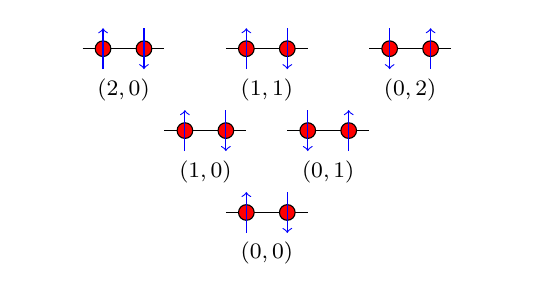
\begin{tikzpicture}[scale=0.52]
                    \draw (-1,0) -- (1,0);
                    \node at (-0.5,0) [draw,circle,fill=red,scale=0.6] {};
                    \node at (0.5,0) [draw,circle,fill=red,scale=0.6] {};
                    \draw[blue, ->] (-0.5,-0.5) -- (-0.5,0.5);
                    \draw[blue, <-] (0.5,-0.5) -- (0.5,0.5);
                    \node[text width=2.2cm, align=center] at (0,-1) {\footnotesize{$(0,0)$}};
                    \draw (-2.5,2) -- (-0.5,2);
                    \node at (-2.0,2) [draw,circle,fill=red,scale=0.6] {};
                    \node at (-1.0,2) [draw,circle,fill=red,scale=0.6] {};
                    \draw[blue, ->] (-2.0,1.5) -- (-2.0,2.5);
                    \draw[blue, <-] (-1.0,1.5) -- (-1.0,2.5);
                    \node[text width=2.2cm, align=center] at (-1.5,1) {\footnotesize{$(1,0)$}};
                    \draw (0.5,2) -- (2.5,2);
                    \node at (1.0,2) [draw,circle,fill=red,scale=0.6] {};
                    \node at (2.0,2) [draw,circle,fill=red,scale=0.6] {};
                    \draw[blue, <-] (1.0,1.5) -- (1.0,2.5);
                    \draw[blue, ->] (2.0,1.5) -- (2.0,2.5);
                    \node[text width=2.2cm, align=center] at (1.5,1) {\footnotesize{$(0,1)$}};
                    \draw (-4.5,4) -- (-2.5,4);
                    \node at (-4.0,4) [draw,circle,fill=red,scale=0.6] {};
                    \node at (-3.0,4) [draw,circle,fill=red,scale=0.6] {};
                    \draw[blue, ->] (-4.0,3.5) -- (-4.0,4.5);
                    \draw[blue, <-] (-3.0,3.5) -- (-3.0,4.5);
                    \node[text width=2.2cm, align=center] at (-3.5,3) {\footnotesize{$(2,0)$}};
                    \draw (-1,4) -- (1,4);
                    \node at (-0.5,4) [draw,circle,fill=red,scale=0.6] {};
                    \node at (0.5,4) [draw,circle,fill=red,scale=0.6] {};
                    \draw[blue, ->] (-0.5,3.5) -- (-0.5,4.5);
                    \draw[blue, <-] (0.5,3.5) -- (0.5,4.5);
                    \node[text width=2.2cm, align=center] at (0,3) {\footnotesize{$(1,1)$}};
                    \draw (4.5,4) -- (2.5,4);
                    \node at (4.0,4) [draw,circle,fill=red,scale=0.6] {};
                    \node at (3.0,4) [draw,circle,fill=red,scale=0.6] {};
                    \draw[blue, ->] (4.0,3.5) -- (4.0,4.5);
                    \draw[blue, <-] (3.0,3.5) -- (3.0,4.5);
                    \node[text width=2.2cm, align=center] at (3.5,3) {\footnotesize{$(0,2)$}};
                \end{tikzpicture}
                \caption{2D with $(n_x,n_y)$}
                \label{subfig:2Dspin}
            \end{subfigure}
            \begin{subfigure}[b!]{0.48\textwidth}
                \centering
                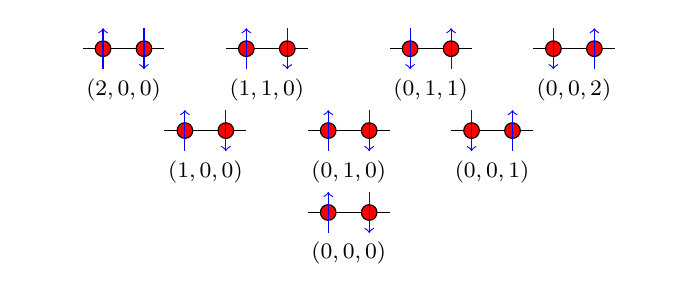
\begin{tikzpicture}[scale=0.52]
                    \draw (-1,0) -- (1,0);
                    \node at (-0.5,0) [draw,circle,fill=red,scale=0.6] {};
                    \node at (0.5,0) [draw,circle,fill=red,scale=0.6] {};
                    \draw[blue, ->] (-0.5,-0.5) -- (-0.5,0.5);
                    \draw[blue, <-] (0.5,-0.5) -- (0.5,0.5);
                    \node[text width=3.5cm, align=center] at (0,-1) {\footnotesize{$(0,0,0)$}};
                    \draw (-4.5,2) -- (-2.5,2);
                    \node at (-4.0,2) [draw,circle,fill=red,scale=0.6] {};
                    \node at (-3.0,2) [draw,circle,fill=red,scale=0.6] {};
                    \draw[blue, ->] (-4.0,1.5) -- (-4.0,2.5);
                    \draw[blue, <-] (-3.0,1.5) -- (-3.0,2.5);
                    \node[text width=2.2cm, align=center] at (-3.5,1) {\footnotesize{$(1,0,0)$}};
                    \draw (-1,2) -- (1,2);
                    \node at (-0.5,2) [draw,circle,fill=red,scale=0.6] {};
                    \node at (0.5,2) [draw,circle,fill=red,scale=0.6] {};
                    \draw[blue, ->] (-0.5,1.5) -- (-0.5,2.5);
                    \draw[blue, <-] (0.5,1.5) -- (0.5,2.5);
                    \node[text width=2.2cm, align=center] at (0,1) {\footnotesize{$(0,1,0)$}};
                    \draw (2.5,2) -- (4.5,2);
                    \node at (3.0,2) [draw,circle,fill=red,scale=0.6] {};
                    \node at (4.0,2) [draw,circle,fill=red,scale=0.6] {};
                    \draw[blue, <-] (3.0,1.5) -- (3.0,2.5);
                    \draw[blue, ->] (4.0,1.5) -- (4.0,2.5);
                    \node[text width=2.2cm, align=center] at (3.5,1) {\footnotesize{$(0,0,1)$}};
                    \draw (-6.5,4) -- (-4.5,4);
                    \node at (-6.0,4) [draw,circle,fill=red,scale=0.6] {};
                    \node at (-5.0,4) [draw,circle,fill=red,scale=0.6] {};
                    \draw[blue, ->] (-6.0,3.5) -- (-6.0,4.5);
                    \draw[blue, <-] (-5.0,3.5) -- (-5.0,4.5);
                    \node[text width=2.2cm, align=center] at (-5.5,3) {\footnotesize{$(2,0,0)$}};
                    \draw (-3.0,4) -- (-1.0,4);
                    \node at (-2.5,4) [draw,circle,fill=red,scale=0.6] {};
                    \node at (-1.5,4) [draw,circle,fill=red,scale=0.6] {};
                    \draw[blue, ->] (-2.5,3.5) -- (-2.5,4.5);
                    \draw[blue, <-] (-1.5,3.5) -- (-1.5,4.5);
                    \node[text width=2.2cm, align=center] at (-2.0,3) {\footnotesize{$(1,1,0)$}};
                    \draw (3.0,4) -- (1.0,4);
                    \node at (2.5,4) [draw,circle,fill=red,scale=0.6] {};
                    \node at (1.5,4) [draw,circle,fill=red,scale=0.6] {};
                    \draw[blue, ->] (2.5,3.5) -- (2.5,4.5);
                    \draw[blue, <-] (1.5,3.5) -- (1.5,4.5);
                    \node[text width=2.2cm, align=center] at (2.0,3) {\footnotesize{$(0,1,1)$}};
                    \draw (6.5,4) -- (4.5,4);
                    \node at (6.0,4) [draw,circle,fill=red,scale=0.6] {};
                    \node at (5.0,4) [draw,circle,fill=red,scale=0.6] {};
                    \draw[blue, ->] (6.0,3.5) -- (6.0,4.5);
                    \draw[blue, <-] (5.0,3.5) -- (5.0,4.5);
                    \node[text width=2.2cm, align=center] at (5.5,3) {\footnotesize{$(0,0,2)$}};
                \end{tikzpicture}
                \caption{3D with $(n_x,n_y,n_z)$}
                \label{subfig:3Dspin}
            \end{subfigure}
            \caption{Harmonic Oscillator Levels}
            \justify
        \end{figure}
    This specific arrangement of basis-functions is implemented in class
    \hltexttt{Cartesian} and is used in both the Hartree-Fock and VMC
    implementations. It essentially builds a matrix of states with the rows
    being the specific state and the columns containing the quantum numbers(in
    cartesian), the spin-value(as an integer), magic number and energy(in
    natural units proportional to the oscillator frequency). The essential form
    is
        \begin{equation}
            \begin{aligned}
                \begin{pmatrix}
                    n_x & n_y & s & m_s & E & M
                \end{pmatrix}
                \indent
                \begin{pmatrix}
                    n_x & n_y & n_z & s & m_s & E & M
                \end{pmatrix}
            \end{aligned}
        \end{equation}
    with the $n$'s being the principal numbers, $s$ the spin value $m_s$ the
    spin projection(up or down in our case), $E$ the energy and $M$ the magic
    number. All the numbers above are integers, meaning the actual energy $E$
    need to be converted if the actual energy of the state is desired, the same
    is applied to the spin projection(which is to multiply by $1/2$). The
    \hltexttt{Cartesian} class builds the states with alternating spin (the
    spacial parts are doubled with spin), but also has a function for
    restructuring by setting the states with spin down in acending order first
    and the same states with spin up after.

\section{Hartree-Fock}
    The Hartree-Fock method described in \Arf{sec:HFtheory} is implemented in
    >> REF GITHUB <<. Only the restricted case is implemented and is present as
    the class \hltexttt{HartreeFockSolver}. The matrix-elements(integrals) are
    implemented in \hltexttt{HermiteIntegrals} class. This class also uses an
    auto-generated header for the Hermite-coefficients, see
    \Arf{sec:auto_generation} below. The \hltexttt{HartreeFockSolver} is
    implemented in a general way such that an abstract class for the integral
    elements is all that is needed. The \hltexttt{HartreeFockSolver} can then
    be inherited and used.  An example of how to create a solver object with
    the Double-Well system called HFS with number of dimensions $D$, number of
    basis functions $L$ and number of particles $N$.
        \begin{lstlisting}[language=C++, style=ccstyle]
            DoubleWell$^*$ HFS = new DoubleWell(D, L, N);
            string message = HFS->initializeParameters(...);
        \end{lstlisting}
    With the $(\dots)$ meaning one initializes it with however manner the
    function was made. The initialization function must also return a message
    determined by the success of the initialization. If it succeeds it returns
    an empty message while if not it returns a pre-defined message. \\ 
    Here is a simple example code-snippet which initializes and runs the
    Hartree-Fock algorithm
        \begin{lstlisting}[language=C++, style=ccstyle]
            DoubleWell$^*$ HFS = new DoubleWell(D, L, N);

            string message = HFS->initializeParameters(...);
            if (message.compare("")) {
                if (myRank == 0) {
                    std::cout << message << std::endl;
                }
                delete HFS;
                finalize();
            }

            double E = HFS->iterate(M, 1e-8, true);
        \end{lstlisting}
    The \hltextttf{iterate} function takes in $M$ as the maximum number of
    iterations, the convergence tolerance (when to break the iteration) and a
    boolean for showing progress or not. It calculates the integral-elements
    and runs the Hartree-Fock algorithm and returns the estimation of the
    ground-state energy.

\subsection{Recurrence Relation and Coefficients}
    The one-dimensional integrals $\xi$(recurrence relation in
    \Arf{eq:recurrInteraction}) 
        \begin{equation}
            \begin{aligned}
                \prd{A_x}[I'_{\text{2D}}] &= -\frac{2\alpha\beta}{\alpha+\beta}
                X_{AB}\zeta_1\left(\frac{\alpha\beta}{\alpha+\beta}R^2_{AB}\right)
                \\
                \xi^n_{00} &= \left(\frac{-2\alpha\beta}{\alpha+\beta}\right)^n
                \zeta_n\left(\frac{\alpha\beta}{\alpha+\beta} R^2_{AB}\right)
            \end{aligned}
        \end{equation}
    involved in the two-body elements and the coefficients
    \Arf{eq:coupledreccoeff}
        \begin{equation}
            \begin{aligned}
                E^{i+1,j}_t &= \frac{1}{2(\alpha + \beta)}E^{ij}_{t-1} -
                \frac{\beta}{\alpha+\beta}(A_x - B_x)E^{ij}_t +
                (t+1)E^{ij}_{t+1} \\
                E^{i,j+1}_t &= \frac{1}{2(\alpha + \beta)}E^{ij}_{t-1} -
                \frac{\alpha}{\alpha+\beta}(A_x - B_x)E^{ij}_t +
                (t+1)E^{ij}_{t+1}
            \end{aligned}
        \end{equation}
    involved in the overlap-distributions in the Hartree-Fock calculations are
    calculated using the class \hltexttt{Hexpander}. The coefficients can be
    calculated and tabulated once with the \hltextttf{setCoefficients}
    function. It is preferable  to set all the needed coefficients once before
    calculating the elements\footnote{Such that precious computation hours are
    not wasted.}. The \hltexttt{Integral} classes all set these in the
    \hltextttf{initializeParameters} function based on the number of
    basis-functions used. For recurrence $\xi$ we implemented a modified
    version of the three-dimensional version by Dragly\cite{draglygithubHF}
    while the $\zeta$ integrals are calculated using
    Gauss-Chebyshev-quadrature\cite{gausschebyshev}. These elements can also be
    tabulated in the same manner as with the coefficients using the function
    \hltextttf{setAuxiliary2D} and \hltextttf{setAuxiliary3D} respectively for
    two- and three dimensions.

    Both the coefficients and integral elements can be obtained with the
    functions \hltextttf{coeff} and \hltextttf{auxiliary2D} and
    \hltextttf{auxiliary3D}.

    In our setup the \hltexttt{Hexpander} class itself is inherited from the
    \hltexttt{GaussianIntegrals} class and used within.

\subsection{Parallelization of Two-Body Matrix}
    The most time-consuming part of the Hartree-Fock procedure is the
    calculation of the two-body matrix-elements giving the interaction terms.
    This is parallelized in the \hltextttf{assemble} function in
    \hltexttt{HartreeFockSolver}. The basic premise is to represent the $N^4$
    elements in $\Braket{pq|r^{-1}|rs}$ as a one-dimensional array with the
    mapping
        \begin{equation}
            (p,q,r,s) \rarr p + N(q + N(r + Ns)).
        \end{equation}
    Which is to say that the element $(p,q,r,s)$ is stored in position $(p +
    N(q + N(r + Ns))$ in the one-dimensional array. The symmetry 
        \begin{equation}
            (p,q,r,s)=(q,p,r,s)
        \end{equation}
    reduces the number of elements down to $N(N+1)/2$. Notice also that the
    number of $(r,s)$ elements each process needs to calculate is also this
    same size meaning the total size is actually
        \begin{equation}
            \text{totalsize} = \frac{N^2(N+1)^2}{4}.
        \end{equation}
    All the symmetries imply that the following elements are the same
        \begin{equation}
            \begin{aligned}
                (p,q,r,s) \\
                (r,q,p,s) \\
                (r,s,p,q) \\
                (p,s,r,q) \\
                (q,p,s,r) \\
                (s,p,q,r) \\
                (s,r,q,p) \\
                (q,r,s,p)
            \end{aligned}
        \end{equation}
    A matrix pqMap of size $N(N+1)/2\times 2$ is then created with elements
        \begin{equation}
            \text{pqMap}_{pq} = (p,q).
        \end{equation}
    This is essentially just a matrix with each row being a tuple with $p$ and
    $q$ value. \\
    The rows are then distributed evenly among $P$ processes according to
    \Arf{eq:divideeven}.
        \begin{equation}
            \text{rows}_{p} = \left\{\begin{aligned}
                \left\lceil\frac{\frac{N}{2}(N+1)}{P}\right\rceil &\indent&
                &\text{rank} < \left(\frac{N}{2}(N+1)\mod P\right) \\
                \left\lfloor\frac{\frac{N}{2}(N+1)}{P}\right\rfloor
                &\indent& &\text{else}
                \end{aligned}\right.
            \label{eq:divideeven}
        \end{equation}
    The problem now however is that processes of higher and higher ranks my end
    up with calculating more since larger indices involve computationally more
    heavy functions to be evaluated. We can account for this by weighting the
    number of rows each process gets by the product\footnote{The product is
    used since the loops are nested and run up to the given quantum number.} of
    the principal quantum numbers for the state which the indices represent,
    that is
        \begin{equation}
            S_i = \suml{j=0}{P_i} \prod_d (n_{j_d}+1).
            \label{eq:Sdefpar}
        \end{equation}
    The sum with index $j$ runs over the sub-chunk for process $i$ where the
    size of each chunk is defined by \Arf{eq:divideeven}.  The algorithm is
    given in \Arf{alg:parasumweight}.
        \begin{algorithm}[H]
            \caption{Even Weighting}\label{alg:parasumweight}
            \begin{algorithmic}[H]
                \State Make an array sizes of size $P$ with the number of
                elements for each process.
                \State Make an array displ of size $P$ with the displacement
                (index).
                \State Make array $S$ of size $P$ with elements as sepcified in
                \Arf{eq:Sdefpar}.
                \State Set elements of sizes array to zero.
                \State $O = $ $\text{Floor}(\text{Mean}(S))$
                \State $p = 0$ \Comment{Index for process}
                \State $j_S = 0$ \Comment{Total sum for each $p$}
                \State $k = 0$ \Comment{Index for displacement in sizes array}
                \State $V_{\text{max}} = O + 3n^2_{\text{max}}$
                \Comment{$n_{\text{max}}$ is the largest $n$-quantum number in
                the system.}
                \For{$l=0$ to $l<\frac{N(N+1)}{2}$} \Comment{Iterate over rows in pqMap}
                    \State $j_S$ = $j_S + \prod\limits_d (n^{(l)}_{p_d}+1)
                    (n^{(l)}_{q_d}+1)$
                    \State $k += 1$
                    \If{$j_S \geq V_{\text{max}}$} \Comment{Make sure not to overshoot}
                        \State sizes$[p] = k-1$ \Comment{Discard the last element}
                        \State $l = l - 1$ \Comment{Re-evaluate for next $p$}
                        \State $k=0$
                        \State $j_S=0$
                        \State $p += 1$
                    \ElsIf{$j_S>O$} \Comment{Chunk for process $p$ is good.}
                        \State $\text{sizes}[p]$ = k \Comment{update sizes}
                        \State $k=0$
                        \State $j_S=0$
                        \State $p += 1$
                    \ElsIf{$l=\frac{N(N+1)}{2}-1$ and $j_S \leq O$}
                    \Comment{Throw remaining rows at last}
                        \State sizes$[p] = k$
                    \EndIf
                \EndFor
            \end{algorithmic}
        \end{algorithm}
    Each process then gets its respective chunk of \hltextttf{pqMap} array such
    that the each process calculates its own chunk according to the size set.
    Each process then calculates the two-body elements with the $(p,q)$
    elements received. The total size for each process also needs to take the
    $(r,s)$ elements into account as they are also of size $N(N+1)/2$. Each
    sub-chunk is then sent to root process and concatenated to a large
    one-dimensional array and the actual two-body matrix of size $N^4$ is
    assembled and antisymmetrized. The Hartree-Fock algorithm is then run only
    on one process.

\subsection{Tabulation of Two-Body Matrix}
    The \hltexttt{HartreeFockSolver} class uses an input file for the two-body
    matrix if given and calculates  and writes one out if not given. As of now
    this is done in a brute-force fashion, that is the entire matrix, including
    all zero-values, are written to file. This entire structure can be improved
    upon by introducing a \txtit{Sparse-Matrix} structure, which is a matrix in
    which only the non-zero elements are stored and a displacement array for
    the given indices of the non-zero elements is created. This would decrease
    the every-increasing memory usage and reduce the calculation time as
    look-up time in the array. \\
    The most promising road for implementing a Sparse structure is to use the
    SparseMatrix module in Eigen since the entire code-base already builds
    heavily upon Eigen from before.

\section{Variational Monte Carlo}
    The Variational Monte-Carlo implementation is mainly in three classes,
    namely \hltexttt{VMC}, \hltexttt{BruteForce} and
    \hltexttt{ImportanceSampling}. The structure is set with
    \hltexttt{BruteForce} and \hltexttt{ImportanceSampling} both inheriting
    from \hltexttt{VMC}. This structure essentially gives room for splitting
    specific parts of the Brute-Force algorithm from the Metropolis-Hastings
    algorithm, but still using the same code for minimization. We will explain
    the minimization parts in the next section. \\ 
    The main input which \hltexttt{VMC} needs is a wavefunction. An abstract
    class-template is implemented and can be generated using a python script,
    also given in the same GitHub repository >>REF GITHUB <<. The template is
    built in such a way that one only needs to fill in specific analytic
    expressions for the gradient, Laplacian and gradient for the variational
    parameters. The latter part is optional. \\ 
    The wavefunction itself is built using the \hltexttt{Slater} or
    \hltexttt{SlaterJastrow} class. However, in order to use the
    \hltexttt{SlaterJastrow} one has to specify which Jastrow function to use
    at compile time. A simple example illustrates this better
        \begin{lstlisting}[language=C++, style=ccstyle]
            SlaterJastrow$^*$ wf = new SlaterJastrow(dim, numParticles, parameters);
            wf->initializeParameters(omega);
            wf->initializeMatrices();

            ImportanceSampling<SlaterJastrow>$^*$ vmc = new
                    ImportanceSampling<SlaterJastrow>(wf, stepmc, parameters,
                                                 maxIterations, rank, numProcs);

            double E = vmc->sampler();

            delete vmc;
            delete wf;
        \end{lstlisting}
    The first chunk initializes the SlaterJastrow class with the pre-specified
    system which needs to be given at compile time as a flag i.e
    WAVEFUNCTION=HARMONICOSCILLATOR. The second part sets the sampling to use
    Metropolis-Hastings algortithm. The parameters variable must be an
    Eigen\cite{eigenweb} vector or array and contain the variational
    parameters. The representation of each element in this vector(or
    array) is specific to each system. For a more detailed explanation see >>
    REF GITHUB <<. \\
    This is just an example of how to build a simple run, however we have also
    built a run file which uses YAML\cite{yaml}. The basic template is as
    follows
        \begin{lstlisting}[language=yaml]
            omega: 1.0
            numparticles: 6
            maxitermc: 100000
            stepmc: 0.01
            parameters: [0.99, 0.47] #optional
            numparameters: 2
            jastrow: true #optional
            importance: true #optional
        \end{lstlisting}
    This is a template used for the \hltexttt{HarmonicOscillator} with the
    Pad\'e-function as Jastrow factor. If the NQS-function is used an
    additional parameter 'numhiddenbias' giving the number of hidden biases
    used, is needed. Again, for more detail see >> REF GITHUB << \\ 
    This form of input makes it fairly simple to actually run the code for
    different systems with ease. One needs to compile with the specific flag
    for the system(wavefunction and Jastrow) and then supply an YAML input file
    at runtime.

\subsection{Statistics}
    Due to the statistical procedure of using a stochastic diffusion process as
    our model there is an inherent variance introduced int the Metropolis
    sampling. In order to get a good estimate for this variance we used the
    method of blocking\cite{blocking}. The implementation is within the class
    \hltexttt{Resampler} in which we have two methods, one called
    \hltextttf{blocking} which effectively reduced the block-sizes and saves
    the variance for each block-size and \hltextttf{autoblocking} which
    estimates the optimal block-size. The latter is taken from the thesis of
    Marius Jonsson\cite{marisugithubblock} and rewritten in \CC using the Eigen
    library.

\subsection{Slater Optimizations\label{susec:slateropt}}
    In the Metropolis sampling we need access to the ratio of two determinants,
    namely the Slater wavefunction at the current state and the one at previous
    state. These are quite expensive to calculate\footnote{Actual complexity of
    a determinant is $\mathcal{O}(n\times n)$, with $n$ being the size of the Slater
    matrix.}. This can be overcome by using the fact that moving only
    \txtit{one} particle at each iteration also constitutes to a
    state-transition. Following \cite{vmc} and given row $i$ as the index for
    the row that is changed, the following expressions are valid
        \begin{equation}
            \begin{aligned}
                \frac{\Psi}{\wtld{\Psi}} &= \sum_j \psi_{ij}
                \wtld{\psi}_{ji}^{-1} \\
                \frac{\nabla_i \Psi}{\Psi} &= \sum_j \psi_{ij} \nabla_i
                \psi_{ji}^{-1} \\
                \frac{\nabla^2_i \Psi}{\Psi} &= \sum_j \psi_{ij} \nabla^2_i
                \psi_{ji}^{-1} \\
            \end{aligned}
        \end{equation}
    with $\wtld{\Psi}$ being the wavefunction at previous state. The
    derivatives all use the wavefunction at current state. One might ask now,
    but isn't this just worse? We have gone from needing two determinants to
    needing two inverses\footnote{!?.}. Fret not, the Sherman-Morrison
    formula\cite{shermorInv} for updating an inverse matrix if only one row has
    changed in the original matrix comes to the rescue. The elements of the
    inverse can by this be expressed as(with $i$ being the row that changed)
        \begin{equation}
            \psi^{-1}_{kj} = \left\{\begin{aligned}
                \wtld{\psi}^{-1}_{kj} -
                \frac{\Psi}{\wtld{\Psi}}\wtld{\psi}^{-1}_{ki}
                \suml{l=1}{N}\psi_{il}\wtld{\psi}^{-1}_{lj}, \indent j \neq i
                \\
                \frac{\Psi}{\wtld{\Psi}}\wtld{\psi}^{-1}_{ki}\wtld{\psi}^{-1}_{ki}
                \suml{l=1}{N}\wtld{\psi}_{il}\wtld{\psi}^{-1}_{lj}, \indent j =
                i
            \end{aligned}\right.
        \end{equation}
    This means that the inverses and the determinant ratios can be calculated
    fully once before the sampling and then updated using the above formulas.
    This procedure is implemented in the \hltexttt{Slater} class.

\subsection{Jastrow Optimizations\label{susec:jastopt}}
    The Jastrow factors presented in \Arf{susec:TWFJastrow},
    \Arf{sususec:TWFPadeJastrow} and \Arf{sususec:NQSJastrow} also give rise to
    optimizations in the case of moving only one particle at a time. In
    particular, the Pad\'e function and the simple exponential can both be
    represented by a matrix of size $N\times D$ like this
        \begin{equation}
            \blds{J} = 
                \begin{pmatrix}
                    \blds{J}(\blds{r}_1) \dots \blds{J}(\blds{r}_N).
                \end{pmatrix}
        \end{equation}
    Moving one particle at a time means only one column in $\blds{J}$ is
    changed meaning only that column needs to be updated. Additionally, the
    $\blds{J}$ matrix doesn't actually need to be present in the code since we
    are only interested in ratios $J/\wtld{J}$. If only one index $i$ changes
    we have
        \begin{align}
            \frac{J}{\wtld{J}} &= \exp(\sumll{i<j} \left(f_{ij} - \wtld{f}_{ij}\right))
            \nonumber \\
            &= \exp(\sumll{i\neq j} f_{ij}).
        \end{align}
    Notice that $i$ is fixed in the last step. \\
    The gradient of $J$ can be represented as an $N\times N\times D$ matrix
        \begin{equation}
            \nabla \blds{J} = 
                \begin{pmatrix}
                    0 & \nabla \blds{J}(\blds{r}_{1,2}) & \dots & \nabla
                    \blds{J}(\blds{r}_{1,N-1}) \\
                    \nabla \blds{J}(\blds{r}_{2,1}) & 0 & \dots & \nabla
                    \blds{J}(\blds{r}_{2,N-1}) \\
                    \vdots & \vdots & \ddots & \vdots \\
                    \nabla \blds{J}(\blds{r}_{N,1}) & \dots & \dots & 0 
                \end{pmatrix}
        \end{equation}
    When only one particle is moved at a time only one row and column changes
    in this matrix. In addition the matrix is symmetric the exception of a sign
    flip
        \begin{equation}
            \nabla \blds{J}(\blds{r}_{ij}) = -\nabla\blds{J}(\blds{r}_{ji}).
        \end{equation}
    Both of these optimizations are implemented in the \hltexttt{PadeJastrow}
    and \hltexttt{ExpNQS} classes. \\ 

    For the NQS-Jastrow we notice that the sum in the exponential involving the
    weights can be represented as a matrix $\blds{W}$ of size $N\times H$ with
    $H$ being the number of hidden biases with elements
        \begin{equation}
            W_{i,j} = \sumll{d}\frac{x^{(d)}_iw_{i+d,j}}{\sigma^2}.
        \end{equation}
    The entire exponential with the hidden biases is represented as a vector
    $\blds{B}$ of size $H$ with elements
        \begin{equation}
            B_j = \exp(b_j + \sumll{i} W_{i,j}).
        \end{equation}
    So for each iteration only one row in $\blds{W}$ is updated and then the
    entire $\blds{B}$ vector is recalculated and reused. \\ 
    The part involving only the visible biases can be optimized in the same
    manner as with the Pad\'e function and simple exponential, meaning one only
    needs to calculate
        \begin{equation}
            \frac{J_a}{J'_a} = \exp(\frac{\left(r_i -
            a_i\right)^2}{\sigma^2}).
        \end{equation}
    Again with $i$ being the index of the moved particle. These optimizations
    are implemented in the \hltexttt{RBMJastrow} class.

\subsection{Optimization For Tabulation\label{susec:optTab}}
    The \hltexttt{Slater} class checks on compile time the specific
    wavefunction class for the functions 
        \begin{itemize}
            \item {\makebox[5cm]{\hltextttf{set}:\hfill} Called during
                initialization (before each sampling)}
            \item {\makebox[5cm]{\hltextttf{reSetAll}:\hfill} Sets all matrices
                to zero (used in testing)}
            \item {\makebox[5cm]{\hltextttf{initializeMatrices}:\hfill}
                Allocate memory}
            \item {\makebox[5cm]{\hltextttf{update}:\hfill} Update positions
                and wavefunction}
            \item {\makebox[5cm]{\hltextttf{reset}:\hfill} Revert to previous
                positions and wavefunction}
            \item {\makebox[5cm]{\hltextttf{resetGradient}:\hfill} Revert to
                previous gradient}
            \item {\makebox[5cm]{\hltextttf{acceptState}:\hfill} Update
                previous positions and wavefunction to current}
            \item {\makebox[5cm]{\hltextttf{acceptGradient}:\hfill} Update
                previous gradient to current one}
        \end{itemize}
    If these functions are implemented in the
    wavefunction class they will be called in by the \hltexttt{VMC} class
    during the Metropolis sampling. The whole purpose for this is so that
    calculations can be tabulated and then only the parts which are changed be
    updated. Detailed explanation of what the functions can, and need to, do is
    given in the GitHub repository.

\subsection{Tabulating Hermite Polynomials}
    In the \hltexttt{HarmonicOscillator} and \hltexttt{HartreeFock} classes
    used by \hltexttt{VMC} we calculate the Hermite polynomials
        \begin{equation}
            \begin{aligned}
                H_n(\sqrt{\omega}r) = \prod_d
                H_{n_d}\left(\sqrt{\omega}x_d\right) \\
                H_n(\sqrt{\omega}r) = \prod_d
                H_{n_d-1}\left(\sqrt{\omega}x_d\right) \\
                H_n(\sqrt{\omega}r) = \prod_d
                H_{n_d-2}\left(\sqrt{\omega}x_d\right)
            \end{aligned}
        \end{equation}
    for $n=0,\dots L$ where $L$ is the number of basis functions in the
    Hartree-Fock basis for \hltexttt{HartreeFock} and highest order of
    single-particle function for \hltexttt{HarmonicOscillator}. These are
    tabulated in a matrix of size $N\times D\times L$ with $N$ being the number
    of particles and $D$. The mapping goes by
        \begin{equation}
            \blds{H}_{ijk} = H_{n^{(d)}_j}\left(\sqrt{\omega}x^{(d)}_i\right).
        \end{equation}
    For each iteration in the Metropolis sampling, if we only move one particle
    at a time, only one row changes in $\blds{H}_{ijk}$. This update is
    reflected in the functions mentioned in \Arf{susec:optTab}.
    \hltextttf{initializeMatrices} firstly allocates space for two matrices
    which represent the current and old versions of $\blds{H}_{ijk}$, the
    \hltextttf{set} function set calculates $\blds{H}_{ijk}$ using the
    auto-generated header explained in \Arf{sec:auto_generation},
    \hltextttf{update} then updates the row which has changed and then
    \hltextttf{acceptState} or \hltextttf{reset} is called depending on the
    Metropolis-Test.

\section{Minimization}
    The central part of the Variational Monte-Carlo method is the actual
    \txtit{variation} of parameters. This is, as explained in \Arf{chapter:3},
    a minimization problem. We will in this chapter explain the implementation
    of the methods presented in \Arf{chapter:5} and also show some examples of
    how to use \hltexttt{Minimizer} class, in which the mentioned methods are
    implemented. \\
    The main class for minimizations is the \hltexttt{Minimizer} and is built
    as a \txtit{friend class}. This is a \CC declaration\footnote{A \CC
    declaration is a phrase which goes in front of variables, functions and
    other objects and is a pure compiler specific rule.} which goes into the
    header of the class who is to befriended (in our case \hltexttt{VMC}) with
    the class who is to be the friend (\hltexttt{Minimizer}). In this way
    \hltexttt{Minimizer} has full access to all the variables and functions
    defined inside \hltexttt{VMC} even if said variables and functions are
    declared as \txtit{private}\footnote{On an equal note, this is truly not a
    good idea in general and great care, inner reflection and utmost scepticism
    must be within the procedural motion of ones thought process before even
    the idea of running forth with such a choice is grasped. It is up for
    discussion if mentioned procedures were completed before the calamity that
    is \hltexttt{Minimizer} was implemented.}. The reason for this choice is
    just to split the whole minimization part of the variational method from
    the actual sampling. \\
    The method are implemented within the following functions
        \begin{itemize}
            \item{\makebox[4cm]{\hltextttf{minimizeSD}\hfill} Gradient Descent.}
            \item{\makebox[4cm]{\hltextttf{minimizeBFGS}\hfill} Quasi-Newton with BFGS and Mor\'e-Thuente linesearch.}
            \item{\makebox[4cm]{\hltextttf{minimizeCG}\hfill} Quasi-Newton with Polak-Ribi\`ere and Mor\'e-Thuente linesearch.}
            \item{\makebox[4cm]{\hltextttf{minimizeASGD}\hfill} Stochastic-Adaptive-Gradient-Descent}
            \item{\makebox[4cm]{\hltextttf{minimizeSABFGS}\hfill} Stochastic-Adaptive method with BFGS.}
            \item{\makebox[4cm]{\hltextttf{minimizeSIAN}\hfill} Simulated Annealing.}
        \end{itemize}
    The specific function is called based on the initial string given to
    \hltexttt{Minimizer} and the means to to make a \hltexttt{Minimizer} object
    is to initialize it as
        \begin{lstlisting}[language=C++, style=ccstyle]
            Minimizer<T>$^*$ m = new Minimizer<T>(vmc, "method", numIterations, eps);
            m$\rarr$minimize();
        \end{lstlisting}
    where \hltexttt{T} is a sampler type (either \hltexttt{BruteForce} or
    \hltexttt{ImportanceSampling}) and \hltextttf{vmc} is the object with said
    type initializes. The \hltextttf{minimize} function is the function which
    actually does the minimization and follows the procedure given in
    \Arf{fig:minimizeProc}.
        \begin{figure}[H]
            \centering
            \begin{tikzpicture}[
                >={Latex[width=2mm,length=2mm]},
                    base/.style = {rectangle, rounded corners, draw=black,
                                minimum width=2cm, minimum height=0.5cm, text
                                centered, font=\sffamily},
                    basecode/.style = {rectangle, rounded corners, draw=black,
                                minimum width=2cm, minimum height=0.5cm, text
                                centered, font=\sffamily, align=left},
                    activityStarts/.style = {base, fill=NavyBlue!30, drop shadow},
                    startstop/.style = {base, fill=Maroon!25, drop shadow},
                    startstopcode/.style = {basecode, fill=Maroon!25, drop shadow},
                    activityRuns/.style = {base, fill=ForestGreen!25, drop shadow},
                    process/.style = {base, fill=white!15, font=\sffamily, drop shadow},
                    processcode/.style = {basecode, fill=white!15, font=\sffamily, drop shadow},
                scale=0.8, 
                node distance=1.5cm, 
                every node/.style={fill=white, font=\sffamily},
                align=center]
                \node (setup) [activityStarts] {
                    Setup \\
                    Initialize vectors for derivatives \\
                    Run \hltexttt{Sampler} \\
                    Save energy given by Sampler
                };
                \node (loop) [startstop, below of=setup, yshift=-0.4cm] {
                    Start loop for $m=0$ to $\text{numIterations}$
                };
                \draw[->] (setup) -- (loop);
                \node (updater) [startstop, below of=loop, yshift=-0.3cm] {
                    call \hltextttf{updater} \\
                    Switch to input method \\
                    if exhausted.
                };
                \node (convergence) [activityRuns, below of=updater, yshift=-0.3cm] {
                    $\abs{\nabla f} \leq \epsilon$
                };
                \node (false) [below of=convergence] {
                   False 
                };
                \node (true) [right of=convergence, xshift=0.6cm] {
                   True 
                };
                \draw[->] (convergence) -- (true);
                \draw[->] (convergence) -- (false);
                \draw[<-] (convergence) -- (updater);
                \draw[->] (loop) -- (updater);
                \node (callFunc) [startstop, below of=false, yshift=-0.2cm] {
                    Save current energy and \\
                    derivatives and \\
                    execute given method
                };
                \node (finish) [activityRuns, below of=callFunc, yshift=-0.2cm] {
                    End
                };
                \draw[->] (true) to [out=0,in=0] (finish);
                \draw[->] (false) -- (callFunc);
                \draw[->] (loop) to [out=0,in=0] (finish);
                \draw[->] (callFunc) to [out=180,in=180] (loop);
            \end{tikzpicture}
            \caption{Flow chart of procedure done by \hltextttf{minimize}
            function.\label{fig:minimizeProc}}
        \end{figure}
    The energy after the last cycle (or after threshold is met) is the energy
    currently saved within the \hltexttt{VMC} object.

\section{Auto-Generation\label{sec:auto_generation}}
\subsection{Hermites}
    The analytic expressions involved in the quantum-dot systems are dependent
    on Hermite polynomials and their coefficients. These are calculated
    symbolically using the recurrence relation for Hermites with the SymPy
    package in python. These expressions are then written to \CC code and
    written to a \CC-header file. The script can be found in
    \url{https://github.com/Oo1Insane1oO/Hermite}. The generated header file is
    then included in the integral class in \hltexttt{HartreeFockSolver} and in
    the wavefunction classes(namely \hltexttt{HartreeFock} and
    \hltexttt{HarmonicOscillator}) in \hltexttt{VMC}.

\subsection{Double-Well Basis}
    The basis built by the procedure described in \Arf{sec:dwfunc} is done in
    python using the eigenvalue solver in the SciPy package. The script itself
    can be found in \url{https://github.com/Oo1Insane1oO/doubleWellFit}, but is
    also included in the Hartree-Fock repository. \\
    The script only builds(calculates the elements of) the $H$ matrix 
        \begin{equation}
            H_{ij} = \veps^{\text{HO}}_i\delta_{ij} +
            \Braket{\psiHO_i|\VDW_n|\psiHO_j},
        \end{equation}
    from \Arf{eq:Heigdef} and then finds its eigenvalues and eigenvectors.
    These are then written to a \CC header file\footnote{Hard-coding the smart
    way} as a class with a static function\footnote{Static means the function
    does not need an object of the container class to be called.} to get
    coefficients and eigenvalues. This file is then included in the
    \hltexttt{DoubleWell} integral class and inherited from.

\section{Verification\label{sec:verification}}
    In order to be confident in the results presented for the double-well
    potential we, along with \txtit{unit-tests}, benchmarked our results with
    the harmonic oscillator potential. The tests are set-up with the
    \pp{UnitTest}\cite{UnitTest++} library and one only needs to pass a flag
    $TESTS=ON$ at compile time to enable them. The benchmark results are given
    in \Arf{tab:HOHF, tab:HOHF3D} >> REF MROE AS YOU GET THEM! <<.

\subsection{Hartree-Fock}
    The first of the test for the Hartree-Fock method was to see if it
    reproduced the exact energies in the case of no interaction(neglect
    Coulomb-term in Hamiltonian). These tests are given in tests directory in
    the GitHub repository.
    
    The benchmarks using the Hartree-Fock method with harmonic oscillator
    potential is given in \Arf{tab:HOHF}. These results are directly compared
    with the master's thesis \cite{lohnethesis} and article
    \cite{hfrefarticle}.
    
    For the double-well system the only benchmark was the result from master's
    thesis of Høgberget\cite{jorgenThesis} with $2$ particles. However it is
    expected that the energies lie somewhere between the single-well results
    and the non-interaction case due to the potential itself being a
    perturbation of the single-well system. The results are given in >> REF(AND MAKE) TABLE <<

\subsection{Variational Monte-Carlo}
    The first tests here were also to find the exact energies, which are also
    given as tests in a similar fashion as with the Hartree-Fock. The second
    benchmark was to check if the energies were comparable with the results of
    \cite{jorgenThesis} using basis functions of form
        \begin{equation}
            \phi_j(\blds{r}) =
            \psi^{\text{HO}}_{n_j}\left(\sqrt{\alpha\omega}r\right),
        \end{equation}
    with the Pad\'e function given in \Arf{eq:padereduceddef}.

    For the real deal with the Hartree-Fock basis we checked that the VMC
    method could reproduce the Hartree-Fock energies when no Jastrow factor was
    used, that is only a single-particle Slater-determinant \txtit{with no
    variational parameters} as the wavefunction ansatz. The expression is
        \begin{equation}
            \phi^{\text{HF}}_{ij} = \sum_l C_{jl}
            \psi^{\text{HO}}_{n_l}\left(\sqrt{\omega}r_i\right).
        \end{equation}
    These results are also implemented as a bunch of tests.

    For the benchmarks, we compared our energies again with the thesis of
    Høgberget\cite{jorgenThesis}. The results are given in >> REF (AND MAKE) TABLE <<

    For the double-well system we only used a Hartree-Fock basis and checked
    that the Hartree-Fock energies were reproduced (in case with no Jastrow).
    The only benchmark was again the system with two particles.
